\section{The discretization}
\label{sec:discr}

In this section we discuss the solution of the Poisson equation in a
domain 
%%
% Widely used methods for the calculation of the space-charge fields are
% the particle-mesh method and the particle-particle method.  The
% particle-mesh method, based on solving Poisson's equation for the
% electrostatic potential, is typically much faster than the
% particle-particle method.  Furthermore, it provides better numerical
% results for sufficiently 'smooth' distributed particles.
%%
\begin{figure}[htb]
  \centering
  % Sketch output, version 0.2 (build 27d, Sat Jan 26 23:58:07 2008)
% Output language: PGF/TikZ
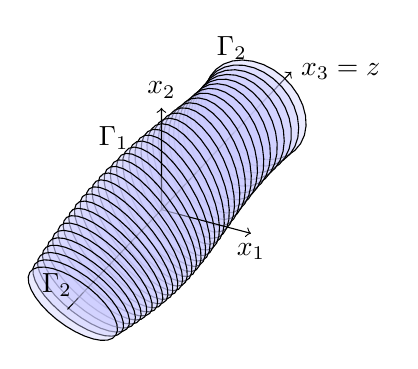
\begin{tikzpicture}[join=round,scale=0.6]
\draw[arrows=->,line width=.4pt](0,0)--(.758,.805);
\filldraw[fill=blue!20,fill opacity=0.4](.584,.697)--(.384,.847)--(.168,.959)--(-.056,1.029)--(-.277,1.055)--(-.487,1.034)--(-.675,.969)--(-.833,.86)--(-.955,.715)--(-1.036,.538)--(-1.071,.337)--(-1.059,.122)--(-1.001,-.099)--(-.899,-.315)--(-.758,-.517)--(-.584,-.697)--(-.384,-.847)--(-.168,-.959)--(.056,-1.029)--(.277,-1.055)--(.487,-1.034)--(.675,-.969)--(.833,-.86)--(.955,-.715)--(1.036,-.538)--(1.071,-.337)--(1.059,-.122)--(1.001,.099)--(.899,.315)--(.758,.517)--cycle;
\draw[arrows=-,line width=.4pt](-.114,-.121)--(0,0);
\filldraw[fill=blue!20,fill opacity=0.4](.38,.658)--(.181,.794)--(-.03,.89)--(-.245,.942)--(-.455,.948)--(-.649,.906)--(-.82,.82)--(-.96,.693)--(-1.064,.531)--(-1.125,.339)--(-1.143,.128)--(-1.115,-.094)--(-1.044,-.317)--(-.932,-.532)--(-.784,-.729)--(-.607,-.899)--(-.409,-1.035)--(-.197,-1.131)--(.018,-1.183)--(.227,-1.189)--(.422,-1.148)--(.593,-1.062)--(.733,-.935)--(.836,-.772)--(.898,-.581)--(.915,-.369)--(.888,-.147)--(.816,.076)--(.705,.291)--(.557,.488)--cycle;
\draw[arrows=-,line width=.4pt](-.227,-.241)--(-.114,-.121);
\filldraw[fill=blue!20,fill opacity=0.4](.175,.613)--(-.021,.735)--(-.227,.815)--(-.432,.849)--(-.629,.835)--(-.808,.774)--(-.961,.668)--(-1.083,.523)--(-1.167,.344)--(-1.21,.14)--(-1.211,-.081)--(-1.168,-.308)--(-1.084,-.533)--(-.962,-.746)--(-.809,-.936)--(-.63,-1.096)--(-.434,-1.218)--(-.228,-1.298)--(-.023,-1.331)--(.174,-1.317)--(.353,-1.256)--(.507,-1.151)--(.628,-1.006)--(.712,-.827)--(.756,-.623)--(.756,-.402)--(.713,-.174)--(.629,.051)--(.508,.263)--(.354,.453)--cycle;
\draw[arrows=-,line width=.4pt](-.341,-.362)--(-.227,-.241);
\filldraw[fill=blue!20,fill opacity=0.4](-.029,.562)--(-.223,.671)--(-.421,.734)--(-.617,.749)--(-.8,.716)--(-.963,.636)--(-1.099,.512)--(-1.201,.35)--(-1.267,.157)--(-1.291,-.059)--(-1.275,-.288)--(-1.217,-.52)--(-1.121,-.746)--(-.991,-.955)--(-.833,-1.137)--(-.653,-1.286)--(-.459,-1.395)--(-.261,-1.458)--(-.066,-1.474)--(.117,-1.44)--(.28,-1.36)--(.416,-1.236)--(.519,-1.074)--(.584,-.881)--(.609,-.665)--(.592,-.436)--(.535,-.204)--(.439,.022)--(.309,.23)--(.15,.413)--cycle;
\draw[arrows=-,line width=.4pt](-.455,-.483)--(-.341,-.362);
\filldraw[fill=blue!20,fill opacity=0.4](-.234,.505)--(-.423,.6)--(-.614,.647)--(-.798,.644)--(-.967,.593)--(-1.114,.494)--(-1.232,.353)--(-1.315,.175)--(-1.362,-.032)--(-1.368,-.258)--(-1.335,-.494)--(-1.263,-.73)--(-1.156,-.955)--(-1.018,-1.159)--(-.856,-1.333)--(-.676,-1.471)--(-.486,-1.565)--(-.296,-1.612)--(-.112,-1.61)--(.057,-1.558)--(.204,-1.46)--(.322,-1.318)--(.406,-1.14)--(.452,-.934)--(.459,-.707)--(.425,-.471)--(.354,-.236)--(.246,-.011)--(.109,.193)--(-.054,.368)--cycle;
\draw[arrows=-,line width=.4pt](-.569,-.603)--(-.455,-.483);
\filldraw[fill=blue!20,fill opacity=0.4](-.437,.443)--(-.622,.523)--(-.805,.553)--(-.977,.533)--(-1.131,.464)--(-1.261,.348)--(-1.36,.19)--(-1.425,-.003)--(-1.453,-.221)--(-1.442,-.457)--(-1.392,-.698)--(-1.307,-.936)--(-1.189,-1.159)--(-1.045,-1.358)--(-.879,-1.524)--(-.7,-1.65)--(-.515,-1.729)--(-.333,-1.76)--(-.16,-1.74)--(-.006,-1.671)--(.124,-1.555)--(.223,-1.397)--(.288,-1.204)--(.316,-.986)--(.304,-.75)--(.255,-.508)--(.17,-.271)--(.052,-.048)--(-.092,.151)--(-.258,.317)--cycle;
\draw[arrows=-,line width=.4pt](-.682,-.724)--(-.569,-.603);
\filldraw[fill=blue!20,fill opacity=0.4](-.639,.373)--(-.819,.439)--(-.992,.454)--(-1.152,.417)--(-1.291,.33)--(-1.404,.197)--(-1.485,.024)--(-1.531,-.182)--(-1.54,-.411)--(-1.512,-.654)--(-1.447,-.901)--(-1.349,-1.139)--(-1.221,-1.359)--(-1.07,-1.552)--(-.903,-1.708)--(-.725,-1.822)--(-.546,-1.887)--(-.373,-1.902)--(-.213,-1.865)--(-.073,-1.778)--(.039,-1.645)--(.12,-1.472)--(.166,-1.267)--(.175,-1.037)--(.147,-.794)--(.082,-.548)--(-.016,-.309)--(-.143,-.089)--(-.294,.104)--(-.462,.26)--cycle;
\draw[arrows=-,line width=.4pt](-.796,-.845)--(-.682,-.724);
\filldraw[fill=blue!20,fill opacity=0.4](-.84,.298)--(-1.013,.349)--(-1.177,.348)--(-1.323,.294)--(-1.447,.191)--(-1.543,.043)--(-1.605,-.144)--(-1.633,-.362)--(-1.624,-.601)--(-1.578,-.851)--(-1.499,-1.1)--(-1.388,-1.338)--(-1.252,-1.555)--(-1.096,-1.74)--(-.927,-1.887)--(-.752,-1.988)--(-.579,-2.039)--(-.415,-2.037)--(-.269,-1.984)--(-.145,-1.881)--(-.049,-1.732)--(.013,-1.545)--(.041,-1.327)--(.032,-1.088)--(-.014,-.839)--(-.093,-.59)--(-.204,-.351)--(-.34,-.135)--(-.496,.051)--(-.665,.197)--cycle;
\draw[arrows=-,line width=.4pt](-.91,-.966)--(-.796,-.845);
\filldraw[fill=blue!20,fill opacity=0.4](-1.039,.216)--(-1.205,.252)--(-1.358,.236)--(-1.491,.166)--(-1.599,.048)--(-1.677,-.115)--(-1.722,-.315)--(-1.731,-.544)--(-1.704,-.791)--(-1.642,-1.046)--(-1.548,-1.297)--(-1.427,-1.533)--(-1.283,-1.745)--(-1.122,-1.923)--(-.952,-2.059)--(-.781,-2.147)--(-.615,-2.183)--(-.462,-2.167)--(-.328,-2.097)--(-.22,-1.979)--(-.142,-1.816)--(-.098,-1.616)--(-.089,-1.387)--(-.116,-1.14)--(-.177,-.886)--(-.271,-.634)--(-.393,-.398)--(-.537,-.186)--(-.697,-.008)--(-.867,.128)--cycle;
\draw[arrows=-,line width=.4pt](-1.023,-1.086)--(-.91,-.966);
\filldraw[fill=blue!20,fill opacity=0.4](-1.235,.127)--(-1.393,.149)--(-1.535,.118)--(-1.655,.033)--(-1.747,-.1)--(-1.808,-.277)--(-1.834,-.488)--(-1.825,-.726)--(-1.781,-.98)--(-1.703,-1.238)--(-1.596,-1.49)--(-1.464,-1.724)--(-1.313,-1.93)--(-1.149,-2.099)--(-.98,-2.224)--(-.812,-2.3)--(-.654,-2.322)--(-.512,-2.29)--(-.392,-2.206)--(-.3,-2.072)--(-.239,-1.896)--(-.213,-1.684)--(-.222,-1.446)--(-.266,-1.192)--(-.343,-.934)--(-.45,-.682)--(-.582,-.448)--(-.734,-.242)--(-.898,-.073)--(-1.067,.052)--cycle;
\draw[arrows=-,line width=.4pt](-1.137,-1.207)--(-1.023,-1.086);
\filldraw[fill=blue!20,fill opacity=0.4](-1.428,.032)--(-1.578,.04)--(-1.709,-.006)--(-1.815,-.105)--(-1.891,-.252)--(-1.934,-.441)--(-1.943,-.663)--(-1.916,-.909)--(-1.855,-1.168)--(-1.763,-1.429)--(-1.643,-1.68)--(-1.501,-1.91)--(-1.344,-2.11)--(-1.177,-2.27)--(-1.009,-2.384)--(-.846,-2.446)--(-.696,-2.454)--(-.565,-2.407)--(-.459,-2.308)--(-.383,-2.161)--(-.34,-1.973)--(-.332,-1.75)--(-.359,-1.504)--(-.419,-1.245)--(-.512,-.985)--(-.631,-.734)--(-.773,-.504)--(-.931,-.304)--(-1.097,-.144)--(-1.266,-.03)--cycle;
\draw[arrows=-,line width=.4pt](-1.251,-1.328)--(-1.137,-1.207);
\filldraw[fill=blue!20,fill opacity=0.4](-1.619,-.07)--(-1.76,-.076)--(-1.879,-.136)--(-1.97,-.249)--(-2.03,-.409)--(-2.056,-.608)--(-2.047,-.84)--(-2.003,-1.092)--(-1.926,-1.355)--(-1.82,-1.617)--(-1.689,-1.866)--(-1.538,-2.092)--(-1.375,-2.284)--(-1.207,-2.434)--(-1.04,-2.536)--(-.883,-2.585)--(-.742,-2.579)--(-.623,-2.519)--(-.531,-2.406)--(-.471,-2.247)--(-.445,-2.047)--(-.455,-1.815)--(-.499,-1.563)--(-.576,-1.3)--(-.682,-1.038)--(-.813,-.789)--(-.964,-.563)--(-1.127,-.371)--(-1.295,-.221)--(-1.461,-.119)--cycle;
\draw[arrows=-,line width=.4pt](-1.365,-1.448)--(-1.251,-1.328);
\filldraw[fill=blue!20,fill opacity=0.4](-1.806,-.178)--(-1.937,-.198)--(-2.044,-.272)--(-2.121,-.397)--(-2.165,-.568)--(-2.174,-.778)--(-2.148,-1.017)--(-2.087,-1.275)--(-1.995,-1.541)--(-1.875,-1.802)--(-1.733,-2.048)--(-1.575,-2.268)--(-1.408,-2.452)--(-1.238,-2.592)--(-1.075,-2.682)--(-.924,-2.718)--(-.792,-2.699)--(-.685,-2.625)--(-.608,-2.499)--(-.564,-2.328)--(-.555,-2.118)--(-.581,-1.879)--(-.642,-1.621)--(-.734,-1.356)--(-.854,-1.094)--(-.996,-.848)--(-1.154,-.628)--(-1.321,-.444)--(-1.491,-.304)--(-1.655,-.214)--cycle;
\draw[arrows=-,line width=.4pt](-1.478,-1.569)--(-1.365,-1.448);
\filldraw[fill=blue!20,fill opacity=0.4](-1.989,-.293)--(-2.111,-.326)--(-2.205,-.412)--(-2.268,-.55)--(-2.296,-.732)--(-2.288,-.95)--(-2.245,-1.196)--(-2.169,-1.458)--(-2.062,-1.725)--(-1.93,-1.985)--(-1.778,-2.226)--(-1.613,-2.439)--(-1.442,-2.614)--(-1.272,-2.744)--(-1.112,-2.822)--(-.968,-2.845)--(-.846,-2.812)--(-.751,-2.725)--(-.689,-2.588)--(-.661,-2.406)--(-.668,-2.187)--(-.711,-1.942)--(-.788,-1.68)--(-.895,-1.413)--(-1.027,-1.153)--(-1.179,-.912)--(-1.344,-.699)--(-1.515,-.524)--(-1.684,-.394)--(-1.845,-.316)--cycle;
\draw[arrows=-,line width=.4pt](-1.592,-1.69)--(-1.478,-1.569);
\filldraw[fill=blue!20,fill opacity=0.4](-2.168,-.414)--(-2.28,-.46)--(-2.362,-.559)--(-2.41,-.707)--(-2.422,-.899)--(-2.398,-1.125)--(-2.339,-1.375)--(-2.247,-1.64)--(-2.127,-1.906)--(-1.983,-2.163)--(-1.822,-2.4)--(-1.651,-2.605)--(-1.478,-2.771)--(-1.309,-2.889)--(-1.153,-2.955)--(-1.016,-2.965)--(-.904,-2.92)--(-.822,-2.821)--(-.774,-2.672)--(-.762,-2.481)--(-.786,-2.255)--(-.845,-2.004)--(-.937,-1.74)--(-1.057,-1.473)--(-1.201,-1.216)--(-1.362,-.979)--(-1.533,-.774)--(-1.707,-.609)--(-1.875,-.49)--(-2.031,-.425)--cycle;
\draw[arrows=-,line width=.4pt](-1.706,-1.81)--(-1.592,-1.69);
\filldraw[fill=blue!20,fill opacity=0.4](-2.344,-.542)--(-2.445,-.599)--(-2.514,-.71)--(-2.547,-.868)--(-2.544,-1.068)--(-2.505,-1.3)--(-2.43,-1.555)--(-2.324,-1.82)--(-2.19,-2.086)--(-2.036,-2.339)--(-1.867,-2.569)--(-1.691,-2.766)--(-1.516,-2.921)--(-1.348,-3.028)--(-1.197,-3.081)--(-1.068,-3.079)--(-.967,-3.022)--(-.898,-2.911)--(-.864,-2.752)--(-.867,-2.553)--(-.907,-2.32)--(-.982,-2.066)--(-1.088,-1.8)--(-1.221,-1.535)--(-1.376,-1.282)--(-1.545,-1.052)--(-1.721,-.855)--(-1.896,-.7)--(-2.063,-.593)--(-2.214,-.54)--cycle;
\draw[arrows=-,line width=.4pt](-1.819,-1.931)--(-1.706,-1.81);
\filldraw[fill=blue!20,fill opacity=0.4](-2.514,-.675)--(-2.605,-.744)--(-2.661,-.866)--(-2.68,-1.033)--(-2.662,-1.24)--(-2.607,-1.477)--(-2.518,-1.734)--(-2.398,-2)--(-2.252,-2.262)--(-2.088,-2.51)--(-1.912,-2.733)--(-1.732,-2.921)--(-1.556,-3.065)--(-1.391,-3.16)--(-1.245,-3.201)--(-1.125,-3.187)--(-1.034,-3.118)--(-.978,-2.997)--(-.959,-2.829)--(-.977,-2.622)--(-1.032,-2.385)--(-1.121,-2.128)--(-1.241,-1.862)--(-1.387,-1.6)--(-1.551,-1.352)--(-1.727,-1.129)--(-1.907,-.941)--(-2.083,-.797)--(-2.248,-.702)--(-2.393,-.661)--cycle;
\draw[arrows=-,line width=.4pt](-1.933,-2.052)--(-1.819,-1.931);
\filldraw[fill=blue!20,fill opacity=0.4](-2.681,-.814)--(-2.76,-.895)--(-2.803,-1.026)--(-2.809,-1.202)--(-2.776,-1.415)--(-2.706,-1.655)--(-2.602,-1.914)--(-2.469,-2.178)--(-2.313,-2.436)--(-2.14,-2.678)--(-1.958,-2.893)--(-1.775,-3.07)--(-1.599,-3.204)--(-1.438,-3.286)--(-1.298,-3.315)--(-1.186,-3.289)--(-1.106,-3.209)--(-1.063,-3.078)--(-1.058,-2.902)--(-1.091,-2.689)--(-1.16,-2.448)--(-1.264,-2.19)--(-1.397,-1.926)--(-1.553,-1.667)--(-1.726,-1.425)--(-1.908,-1.211)--(-2.091,-1.033)--(-2.267,-.9)--(-2.428,-.817)--(-2.568,-.788)--cycle;
\draw[arrows=-,line width=.4pt](-2.047,-2.172)--(-1.933,-2.052);
\draw[arrows=<->,line width=.4pt](-.095,-2.615)--(-1.99,-2.112)--(-1.99,.043);
\filldraw[fill=blue!20,fill opacity=0.4](-2.842,-.959)--(-2.91,-1.05)--(-2.941,-1.19)--(-2.932,-1.373)--(-2.885,-1.591)--(-2.801,-1.834)--(-2.684,-2.092)--(-2.54,-2.354)--(-2.373,-2.607)--(-2.193,-2.842)--(-2.006,-3.047)--(-1.821,-3.214)--(-1.646,-3.336)--(-1.488,-3.407)--(-1.355,-3.423)--(-1.252,-3.385)--(-1.183,-3.294)--(-1.153,-3.155)--(-1.161,-2.972)--(-1.209,-2.754)--(-1.293,-2.511)--(-1.409,-2.253)--(-1.554,-1.991)--(-1.72,-1.737)--(-1.901,-1.503)--(-2.088,-1.298)--(-2.273,-1.13)--(-2.448,-1.009)--(-2.606,-.938)--(-2.739,-.921)--cycle;
\draw[arrows=-,line width=.4pt](-2.161,-2.293)--(-2.047,-2.172);
\filldraw[fill=blue!20,fill opacity=0.4](-2.999,-1.11)--(-3.056,-1.211)--(-3.073,-1.359)--(-3.051,-1.548)--(-2.99,-1.769)--(-2.893,-2.014)--(-2.764,-2.27)--(-2.608,-2.528)--(-2.433,-2.775)--(-2.246,-3.002)--(-2.055,-3.197)--(-1.869,-3.353)--(-1.696,-3.462)--(-1.542,-3.521)--(-1.416,-3.525)--(-1.323,-3.476)--(-1.266,-3.376)--(-1.248,-3.228)--(-1.27,-3.039)--(-1.331,-2.817)--(-1.428,-2.573)--(-1.557,-2.316)--(-1.713,-2.058)--(-1.888,-1.811)--(-2.075,-1.585)--(-2.266,-1.389)--(-2.452,-1.233)--(-2.626,-1.124)--(-2.779,-1.066)--(-2.905,-1.061)--cycle;
\draw[arrows=-,line width=.4pt](-2.274,-2.414)--(-2.161,-2.293);
\filldraw[fill=blue!20,fill opacity=0.4](-3.15,-1.265)--(-3.196,-1.375)--(-3.201,-1.531)--(-3.166,-1.725)--(-3.092,-1.949)--(-2.982,-2.193)--(-2.841,-2.447)--(-2.676,-2.7)--(-2.493,-2.94)--(-2.3,-3.157)--(-2.106,-3.341)--(-1.92,-3.486)--(-1.749,-3.583)--(-1.601,-3.629)--(-1.482,-3.622)--(-1.398,-3.562)--(-1.353,-3.452)--(-1.347,-3.297)--(-1.382,-3.103)--(-1.457,-2.879)--(-1.566,-2.635)--(-1.707,-2.381)--(-1.873,-2.128)--(-2.056,-1.888)--(-2.249,-1.671)--(-2.442,-1.486)--(-2.629,-1.342)--(-2.8,-1.245)--(-2.948,-1.199)--(-3.066,-1.206)--cycle;
\draw[arrows=-,line width=.4pt](-2.388,-2.534)--(-2.274,-2.414);
\filldraw[fill=blue!20,fill opacity=0.4](-3.297,-1.426)--(-3.331,-1.544)--(-3.324,-1.706)--(-3.276,-1.904)--(-3.19,-2.129)--(-3.068,-2.372)--(-2.917,-2.623)--(-2.742,-2.869)--(-2.552,-3.101)--(-2.355,-3.308)--(-2.159,-3.481)--(-1.974,-3.613)--(-1.806,-3.698)--(-1.664,-3.731)--(-1.553,-3.713)--(-1.479,-3.643)--(-1.445,-3.525)--(-1.452,-3.363)--(-1.5,-3.165)--(-1.586,-2.94)--(-1.708,-2.697)--(-1.859,-2.446)--(-2.034,-2.2)--(-2.224,-1.968)--(-2.421,-1.761)--(-2.617,-1.588)--(-2.802,-1.456)--(-2.97,-1.371)--(-3.112,-1.337)--(-3.223,-1.356)--cycle;
\draw[arrows=-,line width=.4pt](-2.502,-2.655)--(-2.388,-2.534);
\filldraw[fill=blue!20,fill opacity=0.4](-3.438,-1.591)--(-3.461,-1.717)--(-3.442,-1.884)--(-3.382,-2.085)--(-3.284,-2.31)--(-3.151,-2.551)--(-2.99,-2.796)--(-2.808,-3.036)--(-2.612,-3.258)--(-2.412,-3.454)--(-2.215,-3.615)--(-2.031,-3.735)--(-1.867,-3.807)--(-1.732,-3.829)--(-1.629,-3.799)--(-1.565,-3.719)--(-1.542,-3.593)--(-1.561,-3.426)--(-1.621,-3.226)--(-1.719,-3)--(-1.852,-2.759)--(-2.013,-2.514)--(-2.195,-2.275)--(-2.391,-2.052)--(-2.592,-1.856)--(-2.788,-1.695)--(-2.973,-1.576)--(-3.136,-1.504)--(-3.272,-1.482)--(-3.374,-1.511)--cycle;
\draw[arrows=-,line width=.4pt](-2.615,-2.776)--(-2.502,-2.655);
\filldraw[fill=blue!20,fill opacity=0.4](-3.574,-1.76)--(-3.586,-1.893)--(-3.556,-2.065)--(-3.484,-2.267)--(-3.375,-2.492)--(-3.232,-2.729)--(-3.062,-2.969)--(-2.873,-3.199)--(-2.673,-3.412)--(-2.47,-3.596)--(-2.273,-3.745)--(-2.091,-3.851)--(-1.933,-3.911)--(-1.804,-3.92)--(-1.71,-3.88)--(-1.656,-3.792)--(-1.645,-3.659)--(-1.675,-3.487)--(-1.747,-3.284)--(-1.856,-3.06)--(-1.999,-2.822)--(-2.168,-2.583)--(-2.358,-2.352)--(-2.558,-2.14)--(-2.761,-1.955)--(-2.958,-1.807)--(-3.139,-1.7)--(-3.298,-1.641)--(-3.427,-1.631)--(-3.521,-1.672)--cycle;
\draw[arrows=-,line width=.4pt](-2.729,-2.897)--(-2.615,-2.776);
\filldraw[fill=blue!20,fill opacity=0.4](-3.705,-1.933)--(-3.707,-2.073)--(-3.665,-2.248)--(-3.582,-2.451)--(-3.462,-2.674)--(-3.31,-2.907)--(-3.133,-3.139)--(-2.938,-3.36)--(-2.734,-3.562)--(-2.53,-3.734)--(-2.334,-3.87)--(-2.156,-3.963)--(-2.002,-4.009)--(-1.881,-4.007)--(-1.796,-3.957)--(-1.753,-3.86)--(-1.752,-3.721)--(-1.793,-3.546)--(-1.876,-3.342)--(-1.996,-3.119)--(-2.148,-2.887)--(-2.325,-2.654)--(-2.52,-2.433)--(-2.724,-2.231)--(-2.929,-2.059)--(-3.124,-1.923)--(-3.303,-1.83)--(-3.456,-1.784)--(-3.577,-1.786)--(-3.662,-1.836)--cycle;
\draw[arrows=-,line width=.4pt](-2.843,-3.017)--(-2.729,-2.897);
\filldraw[fill=blue!20,fill opacity=0.4](-3.831,-2.11)--(-3.822,-2.255)--(-3.769,-2.432)--(-3.676,-2.636)--(-3.547,-2.856)--(-3.387,-3.083)--(-3.203,-3.307)--(-3.003,-3.518)--(-2.796,-3.708)--(-2.592,-3.867)--(-2.398,-3.989)--(-2.224,-4.069)--(-2.077,-4.103)--(-1.963,-4.089)--(-1.888,-4.029)--(-1.854,-3.924)--(-1.864,-3.78)--(-1.916,-3.602)--(-2.009,-3.399)--(-2.139,-3.179)--(-2.299,-2.952)--(-2.483,-2.728)--(-2.683,-2.516)--(-2.889,-2.327)--(-3.094,-2.167)--(-3.288,-2.045)--(-3.462,-1.965)--(-3.609,-1.931)--(-3.723,-1.945)--(-3.798,-2.006)--cycle;
\draw[arrows=-,line width=.4pt](-2.957,-3.138)--(-2.843,-3.017);
\filldraw[fill=blue!20,fill opacity=0.4](-3.952,-2.29)--(-3.932,-2.439)--(-3.869,-2.619)--(-3.767,-2.821)--(-3.629,-3.037)--(-3.461,-3.257)--(-3.272,-3.472)--(-3.068,-3.673)--(-2.86,-3.85)--(-2.656,-3.996)--(-2.465,-4.104)--(-2.296,-4.171)--(-2.155,-4.192)--(-2.05,-4.167)--(-1.984,-4.097)--(-1.961,-3.985)--(-1.981,-3.837)--(-2.044,-3.657)--(-2.146,-3.455)--(-2.285,-3.239)--(-2.452,-3.019)--(-2.642,-2.804)--(-2.845,-2.603)--(-3.053,-2.426)--(-3.257,-2.28)--(-3.448,-2.171)--(-3.617,-2.105)--(-3.758,-2.084)--(-3.863,-2.109)--(-3.929,-2.179)--cycle;
\draw[arrows=-,line width=.4pt](-3.07,-3.259)--(-2.957,-3.138);
\filldraw[fill=blue!20,fill opacity=0.4](-4.068,-2.474)--(-4.038,-2.626)--(-3.965,-2.806)--(-3.854,-3.006)--(-3.708,-3.217)--(-3.534,-3.43)--(-3.34,-3.635)--(-3.134,-3.824)--(-2.925,-3.988)--(-2.723,-4.12)--(-2.536,-4.215)--(-2.372,-4.268)--(-2.239,-4.276)--(-2.142,-4.241)--(-2.086,-4.162)--(-2.072,-4.044)--(-2.103,-3.891)--(-2.175,-3.711)--(-2.287,-3.511)--(-2.433,-3.3)--(-2.607,-3.087)--(-2.801,-2.882)--(-3.007,-2.693)--(-3.215,-2.529)--(-3.418,-2.397)--(-3.605,-2.302)--(-3.768,-2.25)--(-3.902,-2.241)--(-3.999,-2.277)--(-4.055,-2.355)--cycle;
\draw[arrows=-,line width=.4pt](-3.184,-3.379)--(-3.07,-3.259);
\filldraw[fill=blue!20,fill opacity=0.4](-4.179,-2.659)--(-4.139,-2.814)--(-4.057,-2.994)--(-3.937,-3.191)--(-3.784,-3.396)--(-3.605,-3.601)--(-3.408,-3.795)--(-3.2,-3.972)--(-2.992,-4.122)--(-2.793,-4.24)--(-2.61,-4.321)--(-2.452,-4.36)--(-2.327,-4.357)--(-2.239,-4.31)--(-2.192,-4.223)--(-2.189,-4.1)--(-2.229,-3.944)--(-2.311,-3.764)--(-2.431,-3.567)--(-2.584,-3.362)--(-2.763,-3.158)--(-2.96,-2.963)--(-3.168,-2.787)--(-3.376,-2.636)--(-3.576,-2.518)--(-3.758,-2.438)--(-3.916,-2.398)--(-4.041,-2.402)--(-4.129,-2.448)--(-4.176,-2.535)--cycle;
\draw[arrows=-,line width=.4pt](-3.298,-3.5)--(-3.184,-3.379);
\filldraw[fill=blue!20,fill opacity=0.4](-4.285,-2.847)--(-4.236,-3.004)--(-4.145,-3.183)--(-4.018,-3.376)--(-3.859,-3.574)--(-3.675,-3.769)--(-3.475,-3.953)--(-3.267,-4.116)--(-3.061,-4.253)--(-2.865,-4.356)--(-2.688,-4.423)--(-2.537,-4.449)--(-2.42,-4.433)--(-2.341,-4.377)--(-2.304,-4.282)--(-2.31,-4.153)--(-2.36,-3.996)--(-2.45,-3.817)--(-2.578,-3.624)--(-2.737,-3.426)--(-2.92,-3.231)--(-3.12,-3.047)--(-3.328,-2.884)--(-3.534,-2.747)--(-3.731,-2.644)--(-3.908,-2.577)--(-4.058,-2.551)--(-4.176,-2.567)--(-4.255,-2.623)--(-4.292,-2.718)--cycle;
\draw[arrows=-,line width=.4pt](-3.411,-3.621)--(-3.298,-3.5);
\filldraw[fill=blue!20,fill opacity=0.4](-4.387,-3.036)--(-4.328,-3.195)--(-4.23,-3.372)--(-4.096,-3.56)--(-3.931,-3.751)--(-3.745,-3.936)--(-3.543,-4.107)--(-3.336,-4.257)--(-3.132,-4.379)--(-2.94,-4.468)--(-2.769,-4.52)--(-2.626,-4.533)--(-2.517,-4.506)--(-2.448,-4.44)--(-2.42,-4.338)--(-2.436,-4.205)--(-2.494,-4.046)--(-2.593,-3.869)--(-2.727,-3.681)--(-2.891,-3.49)--(-3.078,-3.305)--(-3.28,-3.134)--(-3.487,-2.984)--(-3.691,-2.862)--(-3.883,-2.773)--(-4.054,-2.721)--(-4.197,-2.709)--(-4.306,-2.736)--(-4.375,-2.802)--(-4.403,-2.903)--cycle;
\draw[arrows=-,line width=.4pt](-3.525,-3.741)--(-3.411,-3.621);
\filldraw[fill=blue!20,fill opacity=0.4](-4.484,-3.227)--(-4.417,-3.386)--(-4.311,-3.561)--(-4.171,-3.743)--(-4.002,-3.926)--(-3.813,-4.1)--(-3.611,-4.258)--(-3.405,-4.394)--(-3.205,-4.502)--(-3.019,-4.576)--(-2.854,-4.614)--(-2.719,-4.614)--(-2.62,-4.575)--(-2.559,-4.5)--(-2.541,-4.392)--(-2.566,-4.255)--(-2.633,-4.096)--(-2.739,-3.922)--(-2.88,-3.739)--(-3.048,-3.557)--(-3.237,-3.383)--(-3.439,-3.224)--(-3.645,-3.088)--(-3.845,-2.981)--(-4.032,-2.907)--(-4.196,-2.869)--(-4.331,-2.869)--(-4.431,-2.908)--(-4.491,-2.983)--(-4.509,-3.091)--cycle;
\draw[arrows=-,line width=.4pt](-3.639,-3.862)--(-3.525,-3.741);
\filldraw[fill=blue!20,fill opacity=0.4](-4.576,-3.419)--(-4.502,-3.578)--(-4.389,-3.749)--(-4.244,-3.925)--(-4.072,-4.098)--(-3.881,-4.261)--(-3.68,-4.407)--(-3.477,-4.528)--(-3.281,-4.621)--(-3.1,-4.68)--(-2.943,-4.704)--(-2.817,-4.691)--(-2.727,-4.641)--(-2.676,-4.558)--(-2.667,-4.444)--(-2.701,-4.305)--(-2.776,-4.146)--(-2.889,-3.975)--(-3.034,-3.799)--(-3.206,-3.626)--(-3.397,-3.463)--(-3.598,-3.317)--(-3.801,-3.196)--(-3.997,-3.103)--(-4.177,-3.044)--(-4.334,-3.02)--(-4.461,-3.033)--(-4.551,-3.083)--(-4.602,-3.166)--(-4.61,-3.28)--cycle;
\draw[arrows=-,line width=.4pt](-3.753,-3.983)--(-3.639,-3.862);
\filldraw[fill=blue!20,fill opacity=0.4](-4.665,-3.612)--(-4.583,-3.77)--(-4.464,-3.936)--(-4.314,-4.105)--(-4.14,-4.269)--(-3.949,-4.42)--(-3.749,-4.552)--(-3.549,-4.659)--(-3.359,-4.736)--(-3.185,-4.781)--(-3.036,-4.79)--(-2.919,-4.765)--(-2.838,-4.705)--(-2.797,-4.614)--(-2.798,-4.495)--(-2.84,-4.353)--(-2.923,-4.196)--(-3.041,-4.029)--(-3.191,-3.86)--(-3.365,-3.697)--(-3.556,-3.546)--(-3.756,-3.414)--(-3.956,-3.307)--(-4.146,-3.229)--(-4.32,-3.185)--(-4.469,-3.175)--(-4.586,-3.201)--(-4.667,-3.261)--(-4.708,-3.352)--(-4.707,-3.471)--cycle;
\draw[arrows=-,line width=.4pt](-3.866,-4.103)--(-3.753,-3.983);
\filldraw[fill=blue!20,fill opacity=0.4](-4.75,-3.805)--(-4.66,-3.961)--(-4.536,-4.123)--(-4.383,-4.284)--(-4.207,-4.437)--(-4.017,-4.575)--(-3.819,-4.693)--(-3.624,-4.785)--(-3.44,-4.848)--(-3.274,-4.878)--(-3.133,-4.874)--(-3.025,-4.836)--(-2.954,-4.766)--(-2.923,-4.668)--(-2.932,-4.544)--(-2.983,-4.402)--(-3.072,-4.246)--(-3.196,-4.084)--(-3.349,-3.923)--(-3.525,-3.77)--(-3.716,-3.632)--(-3.913,-3.514)--(-4.108,-3.421)--(-4.293,-3.359)--(-4.459,-3.329)--(-4.599,-3.333)--(-4.707,-3.371)--(-4.779,-3.441)--(-4.81,-3.539)--(-4.8,-3.663)--cycle;
\draw[arrows=-,line width=.4pt](-3.98,-4.224)--(-3.866,-4.103);
\path (.758,.805) node[right] {$x_3 = z$}
                   (-.095,-2.615) node[below] {$x_1$}
                   (-1.99,.043) node[above] {$x_2$};


\node at (-4.2,-3.7) {$\Gamma_2$};
\node at (-3.0,-0.6) {$\Gamma_1$};
\node at (-0.5, 1.3) {$\Gamma_2$};
\end{tikzpicture}% End sketch output

  \caption{Sketch of a typical domain}
  \label{fig:domain}
\end{figure}
%%
$\Omega \subset \Re^3$ as indicated in Figure~\ref{fig:domain}.  The
boundary of the domain is composed of two parts, a curved, smooth
surface $\Gamma_1$ and two planar portions at $z=-d$ and $z=+d$ that
form together $\Gamma_2$.  In physical terms $\Gamma_1$ forms the casing
of the pipe, while $\Gamma_2$ is the open boundary at the inlet and
outlet of the beam pipe, respectively.  The centroid of the particle bunch is at the
origin of the coordinate system.  The Poisson problem that we are going
to solve is given by
\begin{equation} \label{eq:poisson}
  \begin{aligned}
    -\Delta \phi &= \frac{\rho}{\epsilon_0}\ \text{in}\ \Omega, \\
    \phi &= g \equiv 0\ \text{on}\ \Gamma_1,   \\
    \frac{\partial \phi}{\partial \mathbf{n}} + \frac {1}{d} \phi &= 0\
    \text{on}\ \Gamma_2.
  \end{aligned}
\end{equation}
The parameter $d$ in the Robin boundary condition denotes the distance
of the charged particles to the boundary
\cite{poplau_self-adaptive_2008}.  It is half the extent of $\Omega$ in
$z$-direction.  Notice that the Robin boundary condition applies only on
the planar paraxial portions of the boundary.

We discretize~\eqref{eq:poisson} by a second order finite difference
scheme defined on a rectangular lattice (grid)
\begin{displaymath}
  \Omega_h:=\left\{ \mathbf{x} \in {\Omega}\cup\Gamma_2 \ |\ x_i/h_i \in
    \mathbb{Z} \ \mbox{for}\ i=1,2,3 \right\},
\end{displaymath}
where $h_i$ is the grid spacing and $\mathbf{e}_i$ the unit vector in the $i$-th coordinate direction. The
grid is arranged in a way that the two portions of $\Gamma_2$ lie in
grid planes.  A lattice point is called an \emph{interior} point if all
its direct neighbours are in $\Omega$.  All other grid points are called
\emph{near-boundary} points.  At interior points $\mathbf{x}$ we
approximate $\Delta u (\mathbf{x})$ by the well-known 7-point difference
star
\begin{equation}  \label{eq:7pt-star}
  -\Delta_h u(\mathbf{x}) = 
  \sum_{i=1}^3
  \frac{-u(\mathbf{x}\!-\!h_i\mathbf{e}_i) + 2 u(\mathbf{x})
  - u(\mathbf{x}\!+\!h_i\mathbf{e}_i)}{h_i^2}.
\end{equation}
At grid points near the boundary we have to take the boundary conditions
in~\eqref{eq:poisson} into account.  To explain the schemes on the
Dirichlet (or PEC) boundary $\Gamma_1$ let $\mathbf{x}$ be a
near-boundary point.  Let $\mathbf{x}' := \mathbf{x} - h_i\mathbf{e}_i$
for some $i$ be outside $\Omega$ and let $\mathbf{x}^* := \mathbf{x} - s
h_i\mathbf{e}_i$, $0<s\le1$, be the boundary point between $\mathbf{x}$
and $\mathbf{x}'$ that is closest to $\mathbf{x}$,
cf.~Figure~\ref{fig:boundary}.
%%
\begin{figure}[htb]
  \centering
  \input{figures/bdry.pdf_t}
  \caption{1-dimensional sketch of a near-boundary point $x$}
  \label{fig:boundary}
\end{figure}
%%
If $s=1$, i.e., if $\mathbf{x}'\in \partial\Omega$ then $u(\mathbf{x}')$
in~\eqref{eq:7pt-star} is replaced by the prescribed boundary value.
%%
Otherwise, we proceed in one of the three following ways~\cite{fowa:60,
  hack:94}
\begin{enumerate}
\item In \emph{constant extrapolation} the boundary value prescribed at
  $\mathbf{x} - s h_i\mathbf{e}_i \in \Gamma_1$ is assigned to
  $u(\mathbf{x}')$,
  \begin{equation}
    \label{eq:const_extrapol}
    u(\mathbf{x}') = u(\mathbf{x} - h_i\mathbf{e}_i) := g(\mathbf{x}^*).
  \end{equation}
  % Insertion in the five-point difference approximation gives
  % \begin{equation}  \label{eq:5pt-star0}
  %   -\Delta_h^0 u(x,y) = 
  %   \frac{1}{h^2} \left( 4 u_O - g(W^*) - u_S - u_E - u_N \right)
  % \end{equation}
  % This boundary treatment leads to global matrices that are symmetric
  % and positive definite.
\item In \emph{linear extrapolation} the value at $\mathbf{x}'$ is
  obtained by means of the values $u$ at $\mathbf{x}$ and at $\mathbf{x}
  - sh_i\mathbf{e}_i$,
  \begin{equation}
    \label{eq:lin_extrapol}
    u(\mathbf{x}') := (1-\frac{1}{s})\, u(\mathbf{x}) + \frac{1}{s}\,
    g(\mathbf{x}^*).
  \end{equation}
  % This modifies the five-point difference approximation to
  % \begin{equation}  \label{eq:5pt-star1}
  %   \begin{aligned}
  %     -\Delta_h^1 u(x,y) &= \frac{1}{h^2} \left((3+\frac{1}{s})\, u_O -
  %     \right. \\ 
  %     &\quad \left. \frac{1}{s}\, g(W^*) - u_S - u_E - u_N \right).
  %   \end{aligned}
  % \end{equation}
  % \begin{equation}  \label{eq:5pt-star1}
  %   \begin{split}
  %     -\Delta_h^1 u(x,y) =  \\
  %     \frac{1}{h^2} \left((3+\frac{1}{s})\, u_O - \frac{1}{s}\, \right.\\
  %     \left. g(W^*) - u_S - u_E - u_N \right).
  %   \end{split}
  % \end{equation}
  % \begin{equation}  \label{eq:5pt-star1}
  %   -\Delta_h^1 u(x,y) = 
  %   \frac{1}{h^2} \left((3+\frac{1}{s})\, u_O - \frac{1}{s}\,
  %     g(W^*) - u_S - u_E - u_N \right).
  % \end{equation}

% (Note that possibly $\mathbf{x}'\in \partial\Omega$.)

\item \emph{Quadratic extrapolation} amounts to the Shortley-Weller
  approximation~\cite{fowa:60,shwe:39,mcgv:04}.  If $\mathbf{x}'' :=
  \mathbf{x} + h_i\mathbf{e}_i \in \Omega_h$ then the value
  $u(\mathbf{x}')$ is obtained by quadratic interpolation of the values
  of $u$ at $\mathbf{x}$, $\mathbf{x}''$, and the boundary point
  $\mathbf{x}^*$,
  \begin{equation} \label{eq:quad_extrapol}
    u(\mathbf{x}') := \frac{2(s\!-\!1)}{s} u(\mathbf{x}) -
    \frac{s\!-\!1}{s\!+\!1} u(\mathbf{x''}) + %%\\
    \frac{2}{s(s\!+\!1)} g(\mathbf{x}^*).
  \end{equation}
  If $\mathbf{x}'' \not\in \Omega_h$ then let $\mathbf{x}^{**} :=
  \mathbf{x} + t h_i\mathbf{e}_i$, $0<t\le1$, be the boundary point
  between $\mathbf{x}$ and $\mathbf{x}''$ that is closest to
  $\mathbf{x}$.  Then, similarly as before, we get
  \begin{equation} \label{eq:quad_extrapol1}
    \begin{aligned}
      u(\mathbf{x}') &:= \frac{(s\!-\!1)(t\!+\!1)}{st} u(\mathbf{x}) +
      \frac{(t\!+\!1)}{(s\!+\!t)s} g(\mathbf{x}^*) -
      \frac{(s\!-\!1)}{(s\!+\!t)t} g(\mathbf{x}^{**}), \\[1mm]
      u(\mathbf{x}'') &:= \frac{(s\!+\!1)(t\!-\!1)}{st} u(\mathbf{x}) -
      \frac{(t\!-\!1)}{(s\!+\!t)s} g(\mathbf{x}^*) +
      \frac{(s\!+\!1)}{(s\!+\!t)t} g(\mathbf{x}^{**}).
    \end{aligned}
  \end{equation}
 
%   Substituting $u_W$ in~\eqref{eq:5pt-star} gives
%   \begin{equation}  \label{eq:5pt-star2}
%     \begin{aligned}
%       -\Delta_h^2 u(x,y) &=
%       \frac{1}{h^2} \left( (2+\frac{2}{s})\,  u_O -\frac{2}{s + 1}\, u_E
%       \right. \\ 
%       &\quad\ \left. -\frac{2}{(s + 1)s}\, g(W^*) - u_N - u_S \right),
%     \end{aligned}
%   \end{equation}
  %\begin{equation}  \label{eq:5pt-star2}
  %  -\Delta_h^2 u(x,y) = 
  %  \frac{1}{h^2} \left(
  %    (2+\frac{2}{s})\,  u_O
  %    -\frac{2}{s + 1}\, u_E
  %    -\frac{2}{(s + 1)s}\, g(W^*)
  %    - u_N - u_S \right),
  %\end{equation}
\end{enumerate}
In all extrapolation formulae given above we set $g(\mathbf{x}^*) =
g(\mathbf{x}^{**}) = 0$ according to~\eqref{eq:poisson}.  The value on
the right side of~\eqref{eq:const_extrapol}--\eqref{eq:quad_extrapol1}
substitutes $u(\mathbf{x}\! \pm \! h_i\mathbf{e}_i)$
in~\eqref{eq:7pt-star}.

Let us now look at a grid point $\mathbf{x}$ on the open boundary
$\Gamma_2$.  If $\mathbf{x}$ is located on the inlet of the beam pipe
then $\mathbf{x}'':=\mathbf{x}\! +\! h_3\mathbf{e}_3 \in \Omega$ and
$\mathbf{x}':=\mathbf{x}\! -\! h_3\mathbf{e}_3 \not\in \Omega$.  The
Robin boundary condition is approximated by a central difference,
\begin{displaymath}
  - \frac{u(\mathbf{x}'') - u(\mathbf{x}')}{2h_3}
  + \frac{1}{d}u(\mathbf{x}) = 0,
\end{displaymath}
or
\begin{equation}  \label{eq:inlet}
  u(\mathbf{x}') = u(\mathbf{x}'') - \frac{2h_3}{d}u(\mathbf{x}).
\end{equation}
The same formula holds on the outlet boundary portion if $\mathbf{x}'$
denotes the virtual grid point outside $\Omega$.

Notice that some lattice points may be close to the boundary with regard
to more than one coordinate direction.  Then, the
procedures~\eqref{eq:const_extrapol}--\eqref{eq:inlet} must be
applied to all of them.  
% This holds in particular for points on the open
% boundary $\Gamma_2$.

The finite difference discretization just described leads to a system of
equations
\begin{equation} \label{eq:lin-syst}
  A \mathbf{x} = \mathbf{b},
\end{equation}
where $\mathbf{x}$ is the vector of unknown values of the potential and
$\mathbf{b}$ is the vector of the charge density interpolated at the grid
points.
%%
The Poisson matrix $A$ is an $M$-matrix irrespective of the boundary
treatment~\cite{hack:94}.  Constant and linear extrapolation lead to a
\emph{symmetric} positive definite $A$ while quadratic extrapolation
yields a \emph{nonsymmetric} but still positive definite Poisson matrix.

Notice that the boundary extrapolation introduces large diagonal
elements in $A$ if $s$ or $t$ gets close to zero.  In order to avoid
numerical difficulties it is advisable to scale the system matrix.  If
$D = \mbox{diag}{A}$, then we replace $A$ in~\eqref{eq:lin-syst} by
$D^{-1/2} A D^{-1/2}$ and adapt $\mathbf{x}$ and $\mathbf{b}$
accordingly.  


%%% Local Variables: 
%%% mode: latex
%%% TeX-master: "paper"
%%% End: 

